\section{Query Approximation}
\label{sec-query}


Query approximation deals with complex queries involved with big data analytic tasks. Given a class $Q$ of data analytic queries with high a computational complexity,  query approximation is to transform into another class $Q'$ of queries with a low computational complexity and satisfiable approximate answers, as depicted in Fig.~\ref{fig-tech-queryappro} in which $Q$, $Q'$,  $D$ and $R$ denote the original query, approximate query, data and query result, respectively. Query approximation needs to reach a balance between the query efficiency and answer quality when approximating $Q$ with $Q'$.

The rationale behind query approximation lies in that inexact or approximate answers are sufficient or acceptable for many big data analytic tasks.
On one hand, when the volume of data is extremely large, it may be impossible or not necessary to compute the exact answers.
Observe that nobody would try each and every store to find a pair of shoes with the best cost-performance ratio.
That is, inexact (approximate) solutions are good enough in this case.
%
On the other hand, when taking noises (common for big data) into account, it may not always be a good idea to compute exact answers
for those data analytic tasks whose answers are rare or hard to identify, such as the detection of homegrown violent extremists (HVEs) who seek to commit acts of terrorism in the United States and abroad~\cite{HungJ16}, as exact solutions may have a high chance to miss possible candidates.

We next explain query approximation computation in more detail using three different data analytic tasks.



\begin{figure}[tb!]
  \vspace{-1ex}
  \begin{center}
  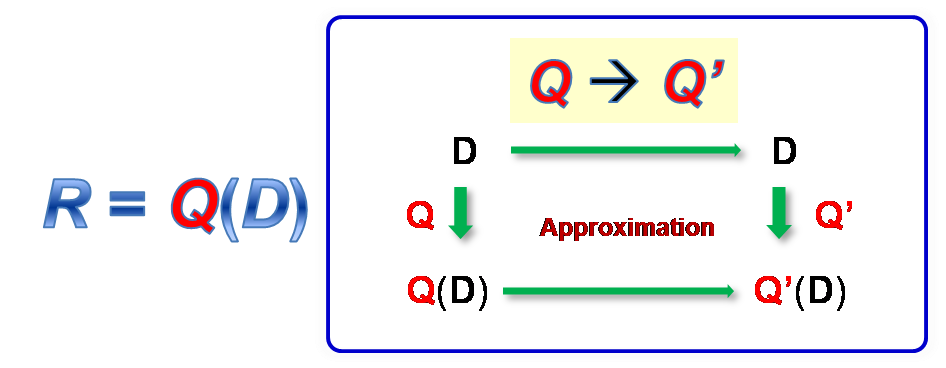
\includegraphics[scale=0.5]{./queryApprox.png}
  \end{center}
  \vspace{-3ex}
  \caption{Query approximation}\label{fig-tech-queryappro}
  \vspace{-2ex}
\end{figure}


\stitle{(1) Strong Simulation~\cite{tods-MaCFHW14}}. Given a pattern graph $Q$ and a data graph $G$,
{\em graph pattern matching} is to find all subgraphs of $G$ that match $Q$, and is being increasingly used in various applications, \eg software, biology, social networks and intelligence analysis.


Here {\em matching} is typically defined in terms of
{\em subgraph isomorphism} \cite{Galla06}:
a subgraph $G_s$ of $G$ {\em matches} $Q$ if
there exists a {\em bijective function} $f$
from the nodes of $Q$ to the nodes in $G_s$ such that (a)  for each
pattern node $u$ in $Q$, $u$ and $f(u)$
have the same label,
and (b) there exists an edge $(u, u')$ in $Q$ if and only
if there exists an edge $(f(u), f(u'))$ in $G_s$.


The goodness of subgraph isomorphism is that all matched subgraphs  are exactly the same as the pattern graph, \ie completely preserving the  topology structure between the pattern graph and data graph. However, subgraph isomorphism is \NP-complete, and may return exponential many matched subgraphs.
Further, subgraph isomorphism is too restrictive to find sensible matches in certain scenarios, as observed in~\cite{FanLMTWW10}. Even worse, online data in many cases only represents a partial world (\eg terrorist collaboration networks and homosexual networks often involve with a large amount of off-line data).
Exact computations on such online data, whose accompanying off-line data is extremely hard to gather, typically decreases the chance of identifying candidate answers.
These hinder the usability of graph pattern matching in emerging applications.


To lower the high complexity of subgraph isomorphism, substitutes for subgraph isomorphism \cite{FanLMTWW10,FanLMTW11}, which allow graph pattern matching to be conducted in cubic-time, have been proposed by extending graph simulation~\cite{infsimu95}. However, they fall short of capturing the topology of data graphs, i.e., graphs may have a structure drastically different from pattern graphs that they match, and the matches found are often too large to analyze.

To rectify these problems, strong simulation, an ``approximate'' substitute for subgraph isomorphism, is proposed for graph pattern matching~\cite{tods-MaCFHW14}, such that strong simulation (a) theoretically preserves the key topology of pattern graphs and finds a bounded number of matches, (b) retains the same complexity as earlier extensions of graph simulation~\cite{FanLMTWW10,FanLMTW11}, by providing a cubic-time algorithm for computing strong simulation, and (c) has the locality property that allows us to develop an effective distributed algorithm to conduct graph pattern matching on distributed graphs.

Strong simulation is experimentally verified that it is able to identify sensible matches that are not found by subgraph isomorphism, and it finds high
quality matches that retain graph topology. Indeed, 70\%-80\% of matches found by subgraph
isomorphism are retrieved by strong simulation. Further, strong simulation is over $100$ times faster than subgraph isomorphism, and has a bounded number of matches.



\stitle{(2) One-Pass Trajectory Compression~\cite{LinMZWH17}}.  Trajectory compression (also known as trajectory simplification) is to compress data points in a trajectory to a set of continuous line segments, and is commonly used  in practice.

Though lossless compression methods incur no information loss, their compression ratios are typically poor, and querying on the compressed data is time consuming due to the reconstruction of the original data \cite{Nibali:Trajic}. Hence, lossy techniques become the mainstream for trajectory compression,
which provide approximate solutions with good compression ratios and bounded errors in practice.


Piece-wise line simplification (\lsa) comes from computational geometry, whose target is to approximate a given finer piece-wise linear curve by another coarser piece-wise linear curve ({normally} a subset of the former), such that the maximum distance of the former from the later is bounded by a user specified constant. It is widely used due to its distinct advantages: (a) simple and easy to implement, (b) no need of extra knowledge and suitable for freely  moving  objects, and (c) bounded errors with good compression ratios.

\lsa algorithms fall into two categories: {\em optimal} and {\em approximate}.
Optimal methods\cite{Imai:Optimal} are to find the minimum number of points or segments to represent the original polygonal lines \wrt an error bound $\epsilon$. They have higher time and space complexities, and are not practical for large trajectory data.
Hence,  various approximate \lsa algorithms have been developed, from batch algorithms (\eg \cite{Douglas:Peucker}) to online algorithms (\eg~\cite{Liu:BQS}) and to one-pass algorithms (\eg~\cite{LinMZWH17}).


An \lsa algorithm is {\em one-pass} if it processes each point in a trajectory once and only once when compressing the trajectory.
Obviously, one-pass algorithms have low time and space complexities, and are more appropriate for online processing. The difficulty comes from the need to achieve effective compression ratios.
Existing trajectory simplification algorithms (\eg \cite{Douglas:Peucker}) and online algorithms  (\eg \cite{Liu:BQS}) essentially employ a global distance checking approach to assuring error bounds, although online algorithms restrict the checking within a window. That is to say, whenever a new directed line segment is formed, these algorithms always check its distances to all or a subset of data points, and, therefore, a data point is checked multiple times, depending on its order in the trajectory and the number of directed line segments formed. Hence, {\em an appropriate local distance checking approach is needed in the first place for designing one-pass trajectory simplification algorithms}.

 We develop a  {\em fitting function} such that a data point is checked only once during the entire process of trajectory simplification. Based on the fitting function, we develop one-pass error bounded trajectory simplification algorithms \operb and \operba that scan each data point in a trajectory once and only once, allowing interpolating new data points or not, respectively. By comparing our algorithms with \fbqsa (the fastest existing \lsa online algorithm \cite{Liu:BQS}) and \dpa (the best existing \lsa batch algorithm in terms of compression ratio \cite{Douglas:Peucker}), our one-pass algorithms  \operb and \operba are over four times faster than \fbqsa, and have  comparable compression ratios with \dpa.


\stitle{(3) Dense Temporal Subgraph Computation~\cite{MaHWLH17}}.  We study dense subgraphs in {\em a special type of temporal networks} such that their nodes and edges are kept fixed, but their edge weights constantly and regularly vary with timestamps~\cite{MaHWLH17}.  Essentially, a temporal network with $T$ timestamps can be viewed as $T$ snapshots of a static network such that the network nodes and edges are kept the same among these $T$ snapshots, while the edge weights vary with network snapthots. Road traffic networks typically fall into this category of temporal networks, and dense subgraphs are used for road traffic analyses that are of particular importance for large cities, such as Beijing, New York, London and Paris, that are facing with heavy traffic congestions, one of the great challenges in urban computing.

Dense subgraphs are a general concept, and their concrete semantics highly depend on the studied problems and applications. Though  dense subgraph discovery and analysis have been widely studied in static networks, how to properly transfer or define their semantics over to temporal networks is still in the early stage, not to mention effective and efficient analytic algorithms.

We adopt the {\em form of dense temporal subgraphs} initially defined and studied in \cite{BogdanovMS11}, such that a temporal subgraph corresponds to a connected subgraph measured by the sum of all its edge weights in a time interval, \ie  a continuous sequence of timestamps. Intuitively, a dense subgraph that we consider  corresponds to a  collection of connected highly slow or jam roads (\ie  a jam area) in road networks, lasting for a continuous sequence of snapshots.


The problem of  finding dense subgraphs in temporal networks is non-trivial, and it is already \NP-complete even for a temporal network with a single snapshot and with $+1$ or $-1$ edge weights only, as observed in \cite{BogdanovMS11}. Even worse, it remains hard to approximate for temporal networks  with single snapshots~\cite{MaHWLH17}. Moreover, given a temporal network with $T$ timestamps, there are a total number of $T*(T+1)/2$ time intervals to consider, which further aggravates the difficulty. The state of the art solution \kw{MEDEN} \cite{BogdanovMS11} adopts a filter-and-verification ({\kw{FAV}) framework that {\em even if a large portion of time intervals are filtered, there often remain a large number of time intervals to verify}. Hence, this method is not big data friendly, and is not scalable when temporal networks have a large number of nodes/edges or a large number $T$ of timestamps.


We develop a data-driven approach, instead of filter-and-verification, to  identifying the most possible $k$ time intervals from $T \times (T + 1)/2$ time intervals, in which $T$ is the number of snapshots and k is a small constant, \eg 10. This is achieved by exploring the characteristics of time intervals involved with dense subgraphs based on the observation of {\em evolving convergence phenomenon} in traffic data, inspired by the convergent evolution in nature\footnote{\small \url{https://en.wikipedia.org/wiki/Convergent_evolution}}. That is, our method provides time intervals with probabilistic grantees, instead of exact ones with \kw{FAV}.   Using both real-life and synthetic data, we experimentally show that Our method \kw{FIDES} is over 1000 times faster than the state of the art solution  \kw{MEDEN}~\cite{BogdanovMS11}, while the quality of dense subgraphs found is comparable with  \kw{MEDEN} .

